\chapter{Implementation}
\label{chapter:implementation}

\section{Introduction}
\label{section:implementation-introduction}

This chapter explores the changes and additions
to the Lex language to include CRE[MFOTL]
refinement from Chapter \ref{chapter:refinement-of-cre-enforcement}.
With refinement in Lex, an existing and possibly fairly abstract
legal formalization can be refined to more closely match
a concrete system.
First we introduce the new language features introduced
for refinement, and then we explore those features in more
detail by refining the EU ePrivacy Directive example
in Lex.

\section{Refinement of Lex Specifications}
\label{section:methodology-refinement-of-lex-specifications}

Refinement introduces a number of new statements in Lex.
Lex refinement files use the file extension \texttt{.rex}.
For refinement, we made the following additions to Lex.
\begin{itemize}
    \item \textbf{Reference to the abstract Lex specification}
        (Keyword: \kw{refine})
        Any Lex refinement specification will start with a \kw{refine}
        statement.
        This statement is simply used to specify the underlying Lex
        specification that is being refined.
        Syntactically it works the same way as an \kw{import} statement
        (e.g. \kw{refine} edp).
    \item \textbf{Event Refinement}
        There are two ways to refine non-internal events in Lex.
        First an event can be marked as assumed to be
        always true or always false,
        and second an event can be refined by
        a combination of other events.
        In the second case, a previously non-internal event
        becomes an internal event in the refined
        specification.
        Section \ref{subsection:lex-event-refinement} dives 
        further into the details of event refinement.
    \item \textbf{Rule strengthening and weakening}
        (Keyword: \kw{replace})
        With refinement, old rules in a Lex specification
        can be replaced by new rules in accordance with
        the implication rules for CRE[MFOTL] refinement
        from Figure \ref{fig:cre-refinement-rules}.
        Section \ref{subsection:lex-rule-strengthening-and-weakening}
        contains more details on the specifics of rule replacement.
    \item \textbf{Type Refinements}
        (Structure: \kw {refine} \kw{type} "abstract type" \kw{is} "concrete type")
        Type refinements are used
        to specify concrete data types for types that
        might have been left abstract in the original
        Lex specification.
        For example, it might be unknown and not necessary
        to know in a legal formalization whether
        a person is represented as a string or integer
        identifier, but in the refinement specification
        we do know which data type is used by the target system.
    \item \textbf{Additional obligations and constitutive rules}
        A refined specification can always contain additional
        obligations that are not explicitly used to
        replace old obligations.
        Similarly, a refined specification can contain
        new constitutive rules that define events which
        may be used anywhere in the refined specification.
        For reasons of simplicity, we have opted to
        disallow the introduction of new exceptions in refined
        specifications, but exception rules can still
        be part of a refinement specification as long
        as they are explicitly used to replace
        existing exceptions.
\end{itemize}

\subsection{Event Refinement}
\label{subsection:lex-event-refinement}
    Refinement rules work almost exactly like constitutive rules.
    The main difference is that the refined event
    in a refinement rule is not an internal event like
    the constituted event in a constitutive rule,
    but it is a non-internal event that gets internalized
    by the refinement.
    The following example shows how this can be expressed as a
    refinement rule.
    Note the use of the \kw{refine} keyword
    to indicate that this is a refinement rule.
    \begin{align*}
        &\kw{rule} \\
        &\quad \kw{whenever} \\
        &\qquad \texttt{consentByEmail(u,s)}~\kw{OR}~\texttt{consentByButton(u,s)} \\            
        &\quad \kw{refine} \\
        &\qquad \texttt{consent(u,s)}
    \end{align*}
    In refinement the conditions must have at least
    the same capability as the refined event.

    Assumptions are in essence syntactic shortcuts for 
    refinement rules that have the condition \kw{true}
    or \kw{false}.
    \begin{align*}
        &\kw{assume}~\bluekw{true}~\texttt{objectToSimilarEmailMarketing}
    \end{align*}
    means that we assume that every user \texttt{u} has objected
    to receiving marketing emails
    from the sender \texttt{s} about products or services in
    category \texttt{c}.
    And this assumption could also be
    written as
    \begin{align*}
        &\kw{rule} \\
        &\quad \kw{whenever} \\
        &\qquad \bluekw{true} \\
        &\quad \kw{refine} \\ 
        &\qquad \texttt{objectToSimilarEmailMarketing(u, s, c)}
    \end{align*}

\subsection{Rule Strengthening and Weakening}
\label{subsection:lex-rule-strengthening-and-weakening}

        Replacement rules are structured and written very similarly to
        other Lex rules.
        They consist of a reference to an old rule
        and one or more references to new rules replacing
        the old one.
        Refinement rules have the form
        \begin{align*}
        & \kw{replace} \\
        & \quad (\kw{strengthen} \mid \kw{weaken}) \\
        & \qquad \text{[old rule reference]} \\
        & \quad \kw{by} \\
        & \qquad \text{[new rule reference(s)]}
        \end{align*}
        Rule replacement is the Lex equivalent to the
        implication (IMP) rules from CRE[MFOTL] in Figure
        \ref{fig:cre-refinement-rules}.

        \textbf{Strengthening Obligations}
        One obligation rule can be replaced by one or
        more obligations that are at least as strong
        as the old obligation.
        Any exception that applied to the old obligation
        will directly apply to the new obligations.
        Weakening of obligations is not allowed, because
        then the refined specification would not correctly
        implement the old one.
        This corresponds to the $\textsc{imp}_R$ rule in
        Figure \ref{fig:cre-refinement-rules}.

        \textbf{Replacing Constitutive Rules}
        A single constitutive rule can be replaced
        by a single constitutive rule and zero
        or more obligations.
        Any exception to the old constitutive rule
        will apply to the new constitutive rule, but
        not the new obligations.
        This corresponds to the $\textsc{imp}_C$ rule
        in Figure \ref{fig:cre-refinement-rules}.
        A constitutive rule can only be strengthened,
        if the constitutive event appears monotonically
        in the old Lex specification, and it can only
        be weakened if the constitutive event appears
        anti-monotonically in the old Lex specification.
        This is condition is necessary, because
        strengthening a constitutive rule means that
        under the stronger rule, the constituted event
        might occur less frequently and under a weaker rule
        it might occur more frequently.
        The (anti) monotonicity condition guarantees that,
        what in essence is the removal (or addition) of
        event occurrences in the refined specification,
        cannot affect whether a trace complies with a
        specification or not.

        \textbf{Replacing Exceptions}
        Analogous to the replacement of constitutive rules,
        a single exception can be replaced by
        a single exception and zero or more obligations.
        This is analogous to the $\textsc{imp}_E$ rule
        in Figure \ref{fig:cre-refinement-rules}.
        Like with constitutive rules,
        the internally created exception event, must
        appear either monotonically or anti-monotonically
        in the old Lex specification such that it can
        be strengthened or weakened respectively.

\section{Implementation in the Lex Compiler}
\label{section:implementation-in-the-lex-compiler}
\begin{figure}
    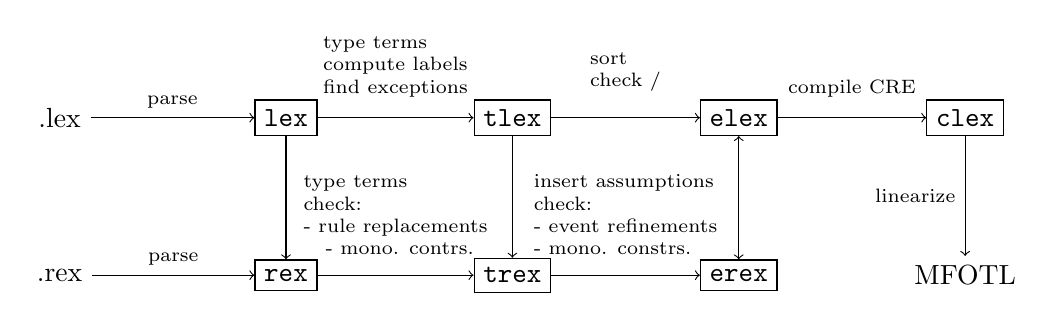
\begin{tikzpicture}
        \node (lex) at (-1.5,0) {.lex};
        \node[draw] (Lex) at (1.375,0) {\texttt{lex}};
        \node[draw] (Tlex) at (4.25,0) {\texttt{tlex}};
        \node[draw] (Elex) at (7.125,0) {\texttt{elex}};
        \node[draw] (Clex) at (10,0) {\texttt{clex}};

        \node (rex) at (-1.5,-2) {.rex};
        \node[draw] (Rex) at (1.375,-2) {\texttt{rex}};
        \node[draw] (Trex) at (4.25,-2) {\texttt{trex}};
        \node[draw] (Erex) at (7.125,-2) {\texttt{erex}};
        \node (WhyEnf) at (10,-2)  {MFOTL};

        \draw[->] (lex) to node[above] {\scriptsize parse} (Lex);
        \draw[->] (Lex) to node[above=4pt,align=left]
            {\scriptsize type terms\\[-4pt]\scriptsize compute labels\\[-4pt]\scriptsize find exceptions} (Tlex);
        \draw[->] (Tlex) to node[above=6pt,align=left]
            {\scriptsize sort\\[-4pt]\scriptsize check $\Cau$/$\Sup$} (Elex);
        \draw[->] (Elex) to node[above=4pt,align=left]
            {\scriptsize compile CRE} (Clex);
        \draw[->] (Clex) to node[left]
            {\scriptsize linearize} (WhyEnf);

        \draw[->] (rex) to node[above]
            {\scriptsize parse} (Rex);
        \draw[->] (Rex) to node[above=4pt,align=left]
            {\scriptsize type terms\\[-4pt]
            %  \scriptsize compute labels\\[-4pt]
             \scriptsize check: \\[-4pt]
             \scriptsize - rule replacements \\[-4pt]
             \scriptsize \quad - mono. contrs.
            } (Trex);
        \draw[->] (Trex) to node[above=4pt,align=left]
            { % \scriptsize check $\refineL_\pi$ \\[-4pt]
             \scriptsize insert assumptions\\[-4pt]
             \scriptsize check: \\[-4pt]
             \scriptsize - event refinements\\[-4pt]
             \scriptsize - mono. constrs.
            } (Erex);
        \draw[->] (Lex) -- (Rex);
        \draw[->] (Tlex) -- (Trex);
        \draw[<->] (Elex) -- (Erex);
    \end{tikzpicture}
    \caption{Structure of the \Lex{} compiler
    \label{fig:lex-compiler} \cite[Figure 13]{lex}}
\end{figure}

We implemented these changes and additions to Lex in the
Lex compiler
\footnote{Lex Compiler \url{https://gitlab.inf.ethz.ch/OU-BASIN/lex/}}.
The changes amount to about 900 lines of OCaml code.
The additions are mainly concentrated in the two files
\texttt{src/rtyping.ml} and \texttt{src/refinement.ml}.
The structure of the Lex compiler is shown in
Figure \ref{fig:lex-compiler}.

The step from \texttt{rex} to \texttt{trex} is implemented
in the \texttt{src/rtyping.ml} file.
In this step terms get type checked, i.e. arguments
to functions and event parameters.
Also section labels get computed.
Finally, the replacement of rules gets checked
on the criteria explained in Section
\ref{subsection:lex-rule-strengthening-and-weakening}.
However, monotonicity depends on the topological ordering,
it can only be determined whether an event appears
monotonically or anti-monotonically in the
Lex specification when all its occurrences in
the specification are known.
Therefore, a set of monotonicity constraints
gets computed in this step and forwarded to the next
step.

The step from \texttt{trex} to \texttt{erex} is implemented
in the \texttt{src/refinement.ml} file.
During this step newly refined events get internalized
and the capabilities of their new definitions get
checked.
Assumptions get unfolded into refinement rules and.
The forwarded monotonicity constraints get checked
based on the topological order.
Also in this step, the "inherited" exceptions from
replaced rules get correctly mapped to the new rules.


